There are two kinds of algebro-geometric objects that have Berkovich spaces associated to them. 
The first one is the analytification of a variety over $K$, analogous to analytification of complex varieties like we discussed in the introduction. 
The second is that there is a natural interpretation of the formal fibre of a formal scheme over $R = \mathcal{O}_K = \{a \in K \st |a| \le 1\} $ as a berkovich space. 


\subsection{Analytification of Vartieties} \label{sec:analytfication_of_vartieties}


Suppose $X$ be a scheme, locally of finite type over $K$.  We want define an analytification functor that takes such schemes to $K$-analytic spaces.  
\begin{definition}
	Let  $X$ be a locally finite $K$-scheme. 
	We define $X\an$ to be the unique $K$-analytic space, together with a morphism of ringed spaces $i: X\an \to X$ such for any good $K$-analytic space $Y$ and morphism of locally ringed spaces $Y \to X$ factors uniquely through $i: X\an \to X$. 
\end{definition}
So $X\an$ represents the functor from $K$-analytic spaces $Y \mapsto \hom(Y, X)$ where the hom-set is in the category of locally ringed spaces. 

This universal property is very useful, but it would be nice to have an more concrete understanding of the analytification of a $K$-variety. 
\begin{definition}\label{def:berkovich_analytification_explicit}
	The \emph{Berkovich analitification} of a locally finite type scheme $X$ over  $K$, as a set is \[
		X\an = \{(x, |\cdot |)  \mid x\in X, |\cdot | \text{ a norm on } k(x) \text{ extending the norm on }K \} 
	.\] 
	\todo{does this need to be smooth and proper and connected?}

	This comes equipped with a cannonical projection map $i: X\an \to X, (x, |\cdot |) \mapsto  x$.
	
	$X\an $ comes with a topology which we define to be the coarsest topology such that 
	\begin{itemize}
		\item $i: X\an \to X$ is continuous, i.e. $X\an$ is a finer space than  $X$. 
		\item For every open $U \subset X$ and $f \in \mathcal{O}_X(U)$ the map  \[
				|f|: i^{-1}(U) \to \R^{+}: (x, |\cdot |) \mapsto  |f(x)|
		\] 
		is continuous.
	\end{itemize}

	\todo{give definition of Berkovich analitification, maybe find an earlier reference than \cite{nicaiseBerkovichSkeletaBirational2016}}
\end{definition}
\todo{is there some definition that also gives $G$-topology and structure sheaf?}

\begin{remark}
	If $X$ is an affine scheme $X = \spec A$ over $K$, then this construction agrees with our adhoc definition from \cref{sec:berkovich_spaces}.
	\[
		X^{\an} = \mathcal{M} (A)
	\] 
	by mapping a norm $x \in \mathcal{M} (A)$ onto $(\ker x, x')$ where $x'$ is the norm on $\kappa(\ker x)$ induced by $x$. 

	We will continue to write $\mathcal{M} (A)$ for the Berkovich analytification of $\spec A$, only this time it inclused the structure sheaf. 
\end{remark}

Like the analytification of Complex varieties there are cetrain GAGA results, which shows that under specific conditions all information is preserved by passing to the Berkovich analytification. 
\todo{write more on GAGA results}


\begin{example}[The Berkovic Affine line $\aff^{1, \text{an}}_K$]
	We already discussed the topology of $\aff^{1, \text{an}}_K$ in \cref{sec:the_berkovich_spectrum_of_z}. 
	But we can now discuss how $\aff^{1, \text{an}}$ behaves as a $K$-analytic space as well. 

	For any $r$ there is a natural inclusion $K[T] \into K\left<r^{-1} T \right>$ and this inclusion is dense. 
	Hence any (semi)norm on $K\left<r^{-1}T \right>$ is uniquely determined by its restriction to $K[T]$.
	Conversely any (semi)norm $|\cdot |_x$ on  $K[T]$ extends to a bounded (semi)norm $K\left<r^{-1}T \right>$ if and only if $r^{-1}|T|_x < 1$, i.e. $|T|_x \le r$. 

	This shows (that as sets at least)
	\[
		\aff^{1, \text{an}}_K = \bigcup_{r = 1} ^{\infty} \mathcal{M} (K\left<r^{-1} T \right>)
	.\] 

\begin{figure}[ht]
    \centering
    \incfig{affine-line-as-union-of-disks}
    \caption{Affine line as union of disks}
    \label{fig:affine-line-as-union-of-disks}
\end{figure}
\end{example}

\begin{example}
	[Berkovich Projective line]
	We can construct the analytification of $\pro^{1}_K$ the same way we construct its spectrum. 
Describe an affine cover $K[T], K[T^{-1}]$ and glue the spaces $\mathcal{M} (K[T]), \mathcal{M} (K[T^{-1})$ along $\mathcal{M} (K[T, T^{-1}])$. 
Using the description in \cref{def:berkovich_analytification_explicit} we see that $\mathcal{M} (K[T, T^{-1}]) = \aff^{1, \text{an}}_K \setminus \{0\} $.
See \cref{fig:berk_projective_line}. 
\end{example}

\begin{figure}[h]
	\centering
	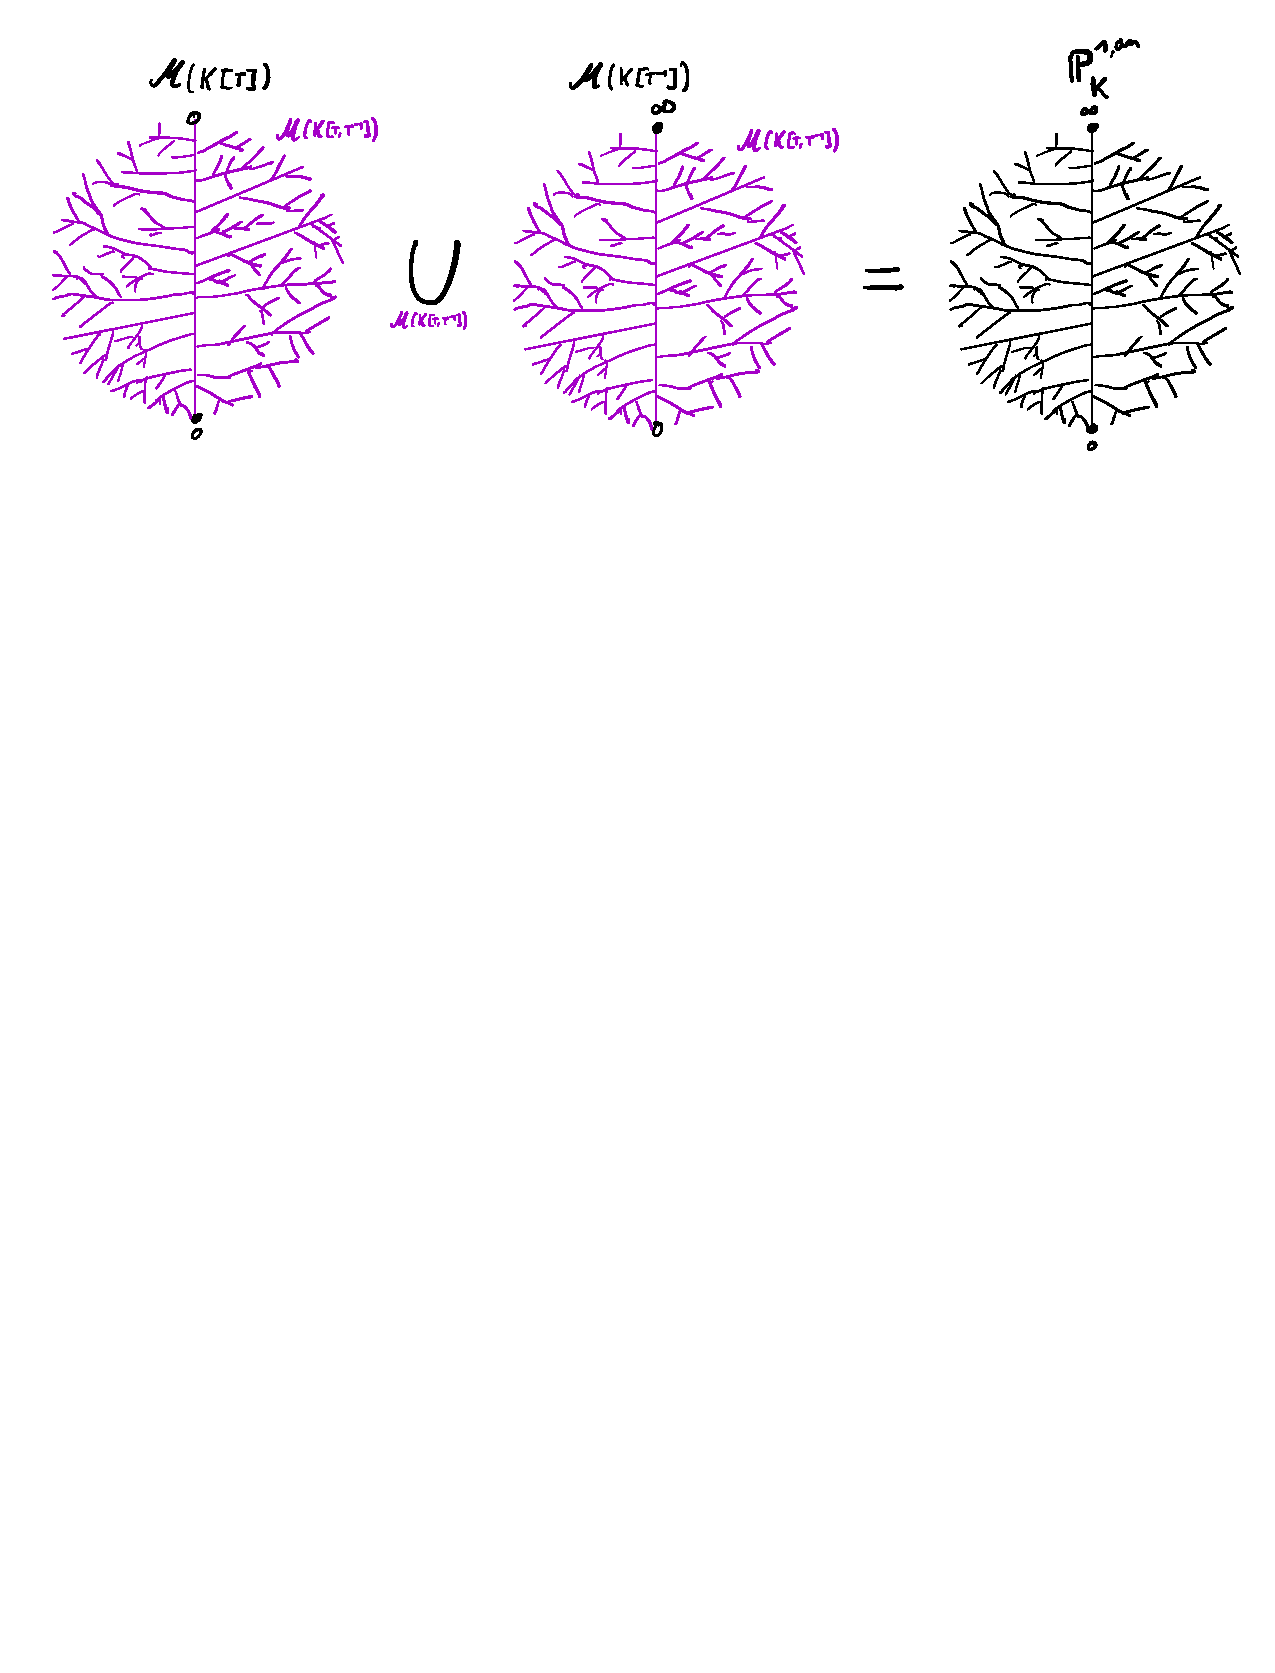
\includegraphics[width=\textwidth]{figures/projective_line}
	\caption{The Berkovich projective constructed by gluing two copies of $\aff^{1, \text{an}}_K$}
	\label{fig:berk_projective_line}
\end{figure}


\subsection{The generic fiber of formal schemes} \label{sec:the_generic_fiber_of_formal_schemes}

Recall that $R = \mathcal{O}_K = \{a \in K \mid a\} $, which is a topological ring with the metric induced by the norm. 
Let $\pi$ be a pseudo-uniformizer for $R$ and $I = (\pi)$. 
Then $\{I^{n}\}_n$ gives a system of neighborhoods around zero, and $R$ is complete with respect to this topology. 
This means that $R$ is an adic ring, which is useful if we want to use the language of formal schemes. 

We first need to restric the class of rings we consider. 

\begin{definition}\label{def:topologically_finite_presentation_algebra}
	A \emph{topologically finitely presented} $R$-algebra is a quotient \[
		R\left<x_1, \ldots, x_n \right> / \mathfrak{a} 
	,\] where $\mathfrak{a}  = (f_1, \ldots, f_m)$ is a finitely generated ideal. 

	A formal scheme that is locally isomorphic to $\spf A$ for some toplogogically finite prestented $R$-algebra is called a \emph{topologically finitely presented} $R$ formal scheme. 
	\todo{check if we need any properties like separated}
\end{definition}

Given such a topologically finitely presented ring $A = \frac{R \left<x_1, \ldots, x_n \right>}{(f_1, \ldots, f_m)}$ we can tensor it with $K$ to get its ``generic fiber'' which is an affinoid algebra \[
A \otimes _R K = \frac{K \left<x_1, \ldots, x_n \right>}{(f_1, \ldots, f_m)}
.\]  
This suggest the following functor $\spf A \mapsto \mathcal{M} (A \otimes_R K)$. 
Indeed this functor glues to give a functor from the topologicically finitely presented $R$ formal schemes to the category of $K$-analytic spaces. 

\begin{definition}\label{def:generic_fibre_of_formal_scheme}
Given a topologically finitely presented formal schemes $\mathfrak{X} $ we call the resulting $K$-analytic space the \emph{generic fibre of  $\mathfrak{X} $} and denote it by $\mathfrak{X} _\eta$. 
\end{definition}

Later we will extend the construction of the generic fibre to the larger class of \emph{special formal schemes}.
\begin{definition}\label{def:special_r_algebra}
	A \emph{special} $R$-algebra is a $R$-algebra of the form \[
		\frac{A\left<x_1, \ldots, x_n \right>[[y_1, \ldots, y_m]]}{(f_1, \ldots, f_\ell)}
	.\] 
\end{definition}

\todo{say something about the reduction map}


